\documentclass[10pt,a4paper,onecolumn]{article}
\usepackage[usenames,dvipsnames]{color}
\usepackage[colorlinks,citecolor=blue]{hyperref}
\usepackage{appendix}
% we need umlauts in the refs
\usepackage[english]{babel}
\usepackage[utf8]{inputenc}
\usepackage[T1]{fontenc}

%\usepackage[natbib=true,style=authoryear,backend=biber]{biblatex}
\usepackage{authblk}
\renewcommand\Affilfont{\itshape\small}
\usepackage{graphicx}
\usepackage[authoryear]{natbib}
\usepackage{url}
\usepackage{todonotes}
%\usepackage{endfloat}
% nicer units
\usepackage{units}
% better tables
\usepackage{booktabs}
% Some colorings for the tables
%\usepackage[table]{xcolor}

%\usepackage{multirow}

% switch for final stage
%\graphicspath{{pics/}}
\graphicspath{{pics/}
              {pics/generated/}}

%\usepackage{lineno}
%\usepackage[leftbars]{changebar}
%\setlength\changebarsep{0.5em}
%\usepackage{comment}

%\usepackage[space]{grffile}
%\usepackage{latexsym}
%\usepackage{amssymb}
%\usepackage{fancyref}
\usepackage{textcomp}

\usepackage{marvosym}
\usepackage{listings}

\lstset{prebreak=\Righttorque}
\lstset{postbreak=\Lefttorque}
\lstset{breakindent=0pt}
\lstset{frame=lines}
\lstset{aboveskip=4mm}
\lstset{breaklines=true, breakatwhitespace=false}
\urlstyle{same}
% howto cite projects
\newcommand{\purl}[2]{#1\footnote{\url{#2}}}

\newcommand{\sevenT}{\unit[7]{Tesla}}
\newcommand{\threeT}{\unit[3]{Tesla}}
\newcommand{\mm}[1]{\unit[#1]{mm}}
\newcommand{\seconds}[1]{\unit[#1]{s}}

\newcommand{\ie}[0]{\emph{i.e.},\ }
\newcommand{\eg}[0]{\emph{e.g.},\ }
\newcommand{\etc}[0]{\emph{etc.}}


\begin{document}
\bibliographystyle{unsrtnat}
\title{Decoding musical genre with an fMRI encoding model of musical
features -- a 3T/7T comparison}


\author[1]{Moritz~Boos}
\author[2]{J.~Swaroop~Guntupalli}
\author[3,4]{Michael~Hanke}

\affil[1]{Oldenburg, Germany}
\affil[2]{Department of Psychological and Brain Sciences,
  Dartmouth College, Hanover, New Hampshire, USA}
\affil[3]{Psychoinformatics lab, Department of Psychology II, University of
Magdeburg, Magdeburg, Germany}
\affil[4]{Center for Behavioral Brain Sciences, Magdeburg, Germany}
\maketitle
\thispagestyle{fancy}

\listoftodos

\begin{abstract}
% Abstracts should be up to 300 words and provide a succinct summary of the
% article. Although the abstract should explain why the article might be
% interesting, care should be taken not to inappropriately over-emphasise the
% importance of the work described in the article. Citations should not be used
% in the abstract, and the use of abbreviations should be minimized.

\todo[inline]{write abstract}
\end{abstract}

\clearpage


\section*{Introduction}

% summary: first comparative study

In functional magnetic resonance imaging (f{MRI}) research, voxel-wise encoding
models are an increasingly popular computational tool to characterize the
relationship between a real world stimulus and BOLD-activity patterns
\citep{NG11,TD+06,KG+08,SZ09}.
A researcher has many choices in building such an encoding model.
Not only parameters of the data analysis, but also parameters of BOLD-acquisition, as field strength and resolution,
might impact encoding performance. \citet{SF14} offer some evidence that an
encoding model performs better on 7-Tesla than 3-Tesla data, but their datasets
did also differ in the number of stimuli used, making it hard to generalize.
Even less is known about effects of feature selection strategies or the choice
of encoding performance metric. Here, we apply three approaches to encoding validation from
different studies and compare them in a 3-Tesla and 7-Tesla dataset with
identical stimuli and comparable design for different data analysis strategies. 

\todo[inline]{what do you think about this 2nd part of an intro paragraph:
need to evaluate the impact of bold acquisition parameters (field strength
resolution -- but little is known about the impact of feature selection
strategies and performance metrics -- there is basically Santoro et al. and
nothing else -- here we explcitely look at things that other studies did
and compare them using a dataset with identical stimuli and comparable design
(in contrast to Santoro?)}
\todo[inline]{How about adding
citations used in the next paragraph? There is a new Neuroimage paper from 
Naselaris as well.-Swaroop}

Encoding models can be validated in a number of different ways: \citet{ML08},
for example, used a binary retrieval task to validate the predicted f{MRI}
images for the meaning of nouns, while \citet{KG+08} used stimulus
identification, and \citet{NG09} used stimulus reconstruction
as a quality metric of encoding performance. In auditory neuroscience, where encoding models are less
frequent, only binary retrieval accuracy \citep{CTK+2012},
%change
which estimates if for each pair of stimuli the predicted data are closer
to the actual data than the switched data, and stimulus
identification \citep{SF14} have been used and it is yet unclear how the
results of these validation strategies vary with the parameters of f{MRI} data
analysis (e.g. number of voxels used)  or acquisition (e.g. field strength).
\citet{SF14} used stimulus identification to validate an encoding model for
natural sounds and reported a difference for 3-Tesla and 7-Tesla f{MRI} data,
although the different number of stimuli used in the two experiments might be a
potential confound.  Apart from field strength, researchers have also many
other degrees of freedom in constructing an encoding model.  Their choice of
parameters, like voxel selection strategy, will affect the quality of
predictions, but it is unknown if these choices will affect encoding quality
metrics differentially.  Recently a 3-Tesla f{MRI} study on the perception of
musical genres \citep{CTK+2012} has been replicated with 7-Tesla data
\citep{HDH+2015}, making it possible to directly compare the effect of field
strength on different validation strategies for encoding models.  This study
aims to compare three quality metrics, binary retrieval accuracy \citep{ML08},
stimulus identification \citep{KG+08,SF14} and the decoding accuracy of a stimulus
feature, the musical genre. We compare
performance on a 3-Tesla and a 7-Tesla dataset while variing the number of
voxels in the model, and the voxel selection strategy.  Although we do
not replicate stimulus reconstruction as in \citep{NG09}, we use a similar
method of constructing a probabilistic decoding model from a set of
voxel-specific encoding models, and use it to infer the music genre of the
presented stimulus.


\section*{Methods}

\subsection*{Stimuli}

origin \citet{CTK+2012}
published in \citet{HDH+2015}

\subsection*{fMRI data}

The analyses presented here were performed on two independently recorded,
and previously published datasets. While these datasets have been acquired
using identical stimuli, with the same number of acquisition runs and
number of stimulation trials, they nevertheless differ in their precise
stimulation timing, stimulation setup and equipment, as well as other
acquisition details. A brief description of both datasets is provided below.
For more information the reader is referred to the respective publications.

\paragraph{\unit[3]{Tesla}}
%
\todo[inline]{Swaroop, please add a brief summary and at least one citation}

\paragraph{\unit[7]{Tesla}}
%
\citet{HDH+2015}; maybe \citet{HBI+14}


\subsection*{Preprocessing}

Temporal lobe masks for each participant were extracted from Montreal
Neurological Institute coordinate space using FSL \citep{SJB+04,JBB+12}.
Each voxel inside the temporal lobe mask was run-wise normalized and linearly
de-trended using PyMVPA \citep{HHS09b}. 

\subsection*{Encoding model}

To build an encoding model with high predictive power, we need to find an
appropriate feature representation of the music stimuli.  \citet{CTK+2012}
already compared different feature representations of the same stimuli in the
3T dataset. They found that features corresponding to the timbre of the stimulus
performed best.
We chose a similar feature set made available by \citet{HDH+2015}, the low-quefrency
mel-frequency spectrum (LQ-MFS).


\begin{figure}
  \centering
  \includegraphics[width=\linewidth]{pics/encoding_scheme}

  \caption{A schematic overview of the encoding process. The spectrogram for
	  each stimulus is transformed into its low-quefrency mel-frequency
	  spectrum (LQ-MFS). Then, the encoding features are extracted by a
  sliding window from the LQ-MFS. Using these features, encoding model is trained on all runs in
  the training set, and used to predict the f{MRI} activity of the left-out run.
  These predictions are subsequently used for validation.}

 \label{fig:encoding_scheme}
\end{figure}


For each f{MRI} sample $y_{vt}$ (where $t=1,2,..,T$ denotes the time-points and
$v=1,2,..,V$ denotes the voxels) the LQ-MFS features $x_{t}$ $[1\times\widetilde{M}]$
(where $\widetilde{M}$ is the number of LQ-MFS coefficients) of the
corresponding two second part of the stimulus were computed. In case there was
no stimulus presented at time-point $t$, a zero vector $[1\times\widetilde{M}]$ was
used. 

Since the BOLD response is delayed,  the most recent feature vector was removed
for each f{MRI} sample (since it could not yet have influenced the f{MRI}
activity), and the new feature vector at time-point $t$ was created by
concatenating the prior feature vectors $x_{t-1}$,$x_{t-2}$ and $x_{t-3}$. We
overload \todo{dunno what this mean? jargon?} the notation and denote this stacked feature vector as $x_{t}$.
Feature vectors (and the corresponding f{MRI} sample) were removed from the
analysis, if two-thirds or more of the concatenated feature vectors were
zero-vectors.

The f{MRI} activity time-series, as well as the feature time-series, were
vertically stacked, resulting in a matrix of features $X$ $[N\times M]$ (where $N$ is
the number of f{MRI} samples, and $M$ is number of LQ-MFS coefficients, with
$M=3\widetilde{M}$) and a matrix of f{MRI} activity $Y$ $[N\times V]$ (where $V$ is
the number of voxels).

%probabilistic or objective function minimization, also cite someone about using lin. reg. in encoding
The encoding model could then be expressed as the probability to observe the f{MRI} activity at time-point $t$ and voxel $v$:
%
\begin{equation}
  \label{eq:encmo}
  p(y_{vt}|x_{t}) = N(y_{vt};x_{t}\beta_{v},\sigma)
\end{equation}
%
where $N(y;\mu,\sigma)$ denotes the probability density at point $y$ for a
Gaussian with mean $\mu$ and standard deviation $\sigma$, and $\beta_{v}$ is a
$[M\times1]$ vector of regression coefficients specific to voxel $v$. To reduce
over-fitting, the regression-coefficients were estimated using ridge regression
\citep{HK70}.  Independently for each voxel, the regularization parameter
$\lambda$ with the lowest mean squared error in a generalized leave-one-out
cross-validation \citep{GHW79} was chosen from a set of candidate values.

\subsection*{Quality metrics} 

\paragraph{Binary retrieval accuracy}

Binary retrieval accuracy \citep{ML08} estimates if a stimulus'
predicted f{MRI} activity is closer, in terms of cosine similarity, to its
observed f{MRI} activity than to the f{MRI} activity of a decoy stimulus.
This is done pair-wise for all combinations of stimuli, include stimuli from the
same genre, and then averaged.

In a prior study \citep{CTK+2012}, using the 3-Tesla data, binary retrieval
accuracy was used to validate voxel-specific encoding models on the same
dataset.

\paragraph{Correlation rank score}
%
An alternative measure of encoding performance is the correlation rank score or
matching score \citep{SF14}. For each stimulus $s_{n}$ in the validation set,
its predicted f{MRI} activity $\widetilde{y}_{n}$ is correlated with the
observed f{MRI} activity of every stimulus, $y_{i}$ for $i=1..25$. These
correlations are then ordered, and the  matching score $m(s_{n})$ is \[
m(s_{n}) = 1-\frac{rank(s_{n})-1}{N-1} \] Where $rank(s_{n})$ is the rank of
the correlation between predicted $\widetilde{y}_{n}$ and observed $y_{n}$
f{MRI} activity of $s_{n}$. Finally, the matching scores for all stimuli in the
validation set are averaged.


\paragraph{Decoding of stimulus category}

\begin{figure}
  \centering
  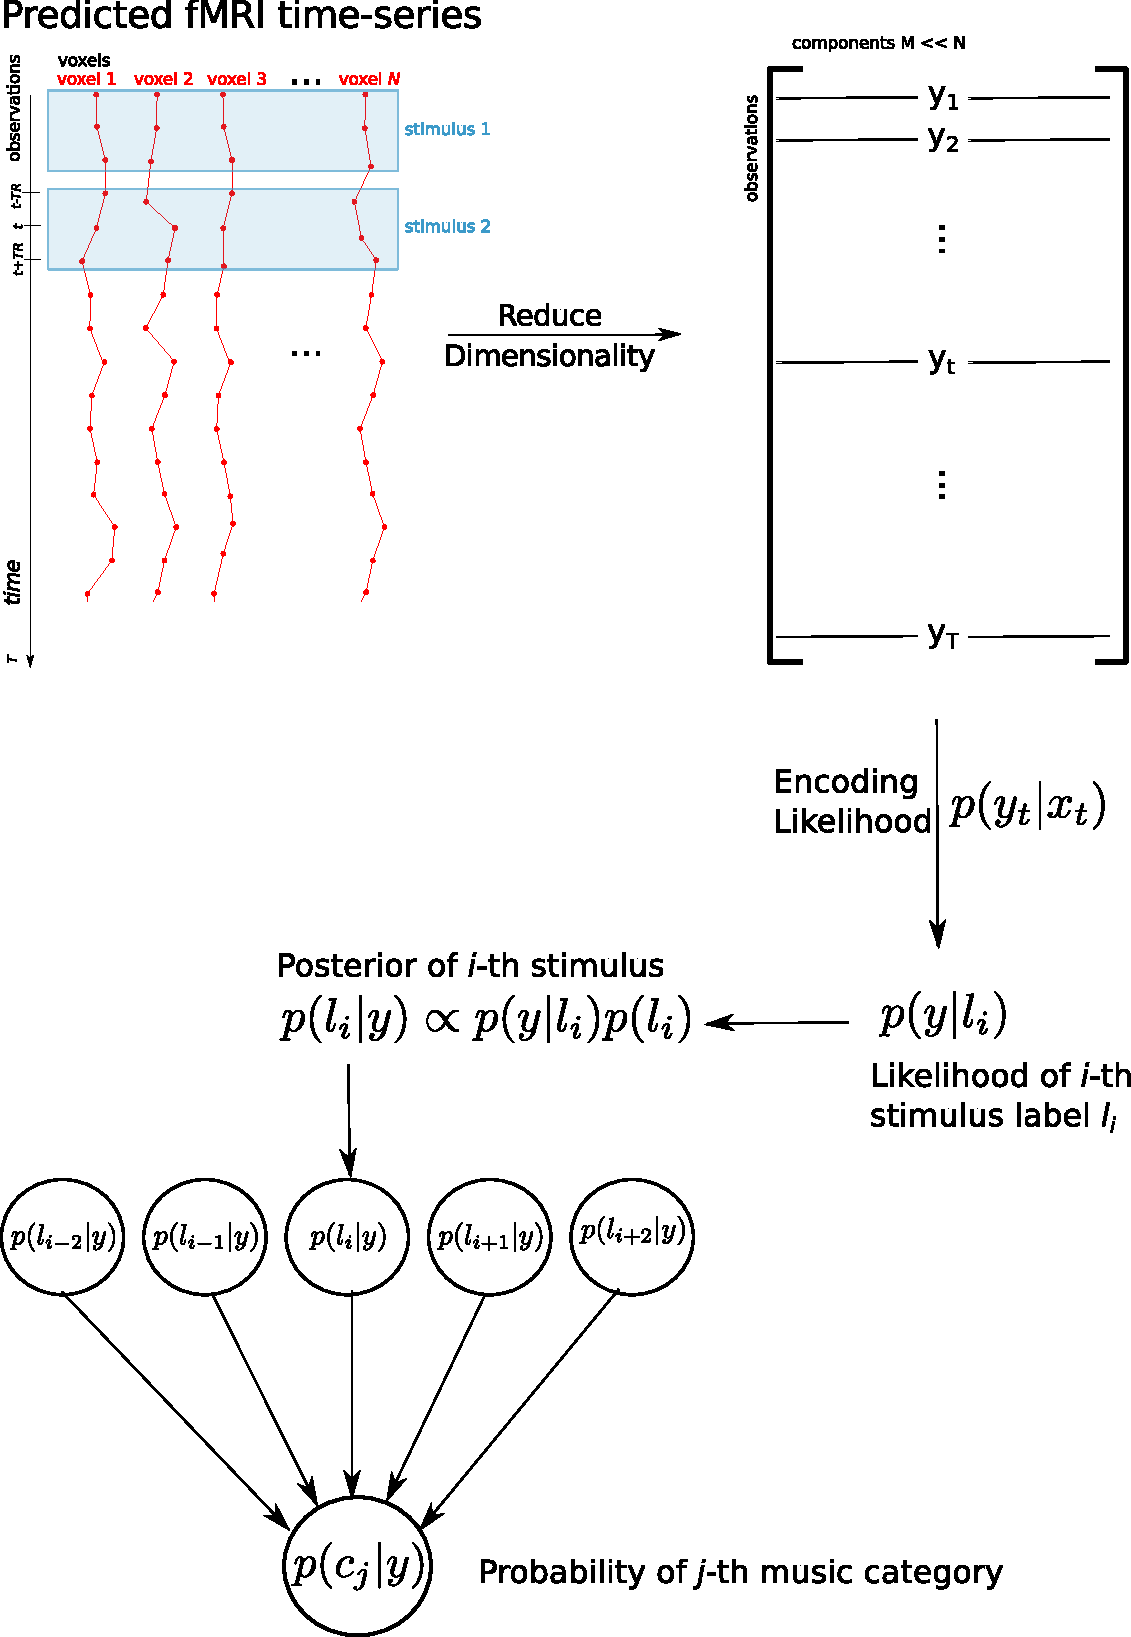
\includegraphics[width=\linewidth]{pics/Decoding_scheme}

  \caption{A schematic overview of the decoding of music category. The predicted
  f{MRI} time series of the validation run is reduced in dimensionality by
  principal component analysis,
  and a multivariate-normal likelihood function $p(y_{t}|x_{t})$ is constructed.
  From there, the probability distribution over music stimuli and subsequently musical categories is estimated.}

 \label{fig:decoding_scheme}
\end{figure}


Instead of testing the encoding performance, we can also test the performance of
a decoder based on the individual encoding models \citet{NG11}
(Figure \ref{fig:decoding_scheme}). To go from
$p(y_{vt}|x_{t})$ to $p(x_{t}|y_{t})$ we follow \citet{NG09} and first condense
the large number of voxel-specific encoding models into one multi-voxel encoding model.
To do this we project the predicted and observed f{MRI} data onto the first $k$
principal components of the $[N\times V]$ matrix of predicted f{MRI} activity, where $k$ is the number of principal components that maximize the decoding
accuracy on the training set for this participant.
As in \citet{NG09} we construct the $k$-dimensional multivariate normal
probability density function $p(y_{t}|x_{t})$ to obtain a likelihood function across voxels.
To build a decoding model, we now express this likelihood in terms of the label
of the music stimulus instead of its LQ-MFS features.
We use the simplifying assumption that the f{MRI} activity is influenced by the music stimuli only through their LQ-MFS
coefficients $x$, and --- given that each music stimulus was associated with only
three (lagged) LQ-MFS representations --- the likelihood to observe a given
triple of consecutive $y$ for a specific music stimulus $l_{i}$ is $p(y|l_{i}) \propto
p(y_{t-1}|x_{1})p(y_{t}|x_{2})p(y_{t+1}|x_{3})$ where $t$ is the sample 6
seconds after the start of the music stimulus and $x$ are the three LQ-MFS
feature vectors of this stimulus.
For a given triple of consecutive f{MRI} activity $y$ from the same stimulus, we can now estimate the probability distribution over music stimuli
$p(l_{i}|y)$ (for $i=1..25$) by using Bayes' rule: $p(l_{i}|y) \propto
p(y|l_{i})p(l_{i})$ and ignoring the normalizing constant $p(y)$. Since each
stimulus was presented was presented exactly once, it has an uniform prior
distribution with $p(l_{i})=\frac{1}{25}$. The mode of this distribution is the
most probable presented stimulus given the data.
We can then decode the musical genre of the presented stimulus given the observed f{MRI} activity as the mode of $p(c_{i}|y)
\propto \prod\nolimits_{l \in stim(c_{i})} p(l|y)$ where $stim(c_{i})$ are
the labels of the stimuli belonging to the genre $c_{i}$. 

\subsection*{Voxel selection}

We varied the number of voxels used in the analysis, both for 3- and 7-Tesla f{MRI} data,
and selected which voxels to keep by two different criteria. Both criteria were
based on voxel characteristics in the training set.  

\paragraph{Selection by stability}

\citet{ML08} selected the 500 most stable voxels for their analysis. For one
voxel, each run can be represented as a vector of f{MRI} activity, where each
entry is associated with one stimulus. A voxel's "stability score" is the average correlation between the vectors of the 25 stimuli's f{MRI} activity of each pair of runs.
This criterion selects voxels with consistent activation for each stimulus across runs.

\paragraph{Selection by $r^2$}

Since we are interested in encoding performance, we can use the quality of
predictions of each voxel's encoding model as a selection criterion. We compute
the coefficient of determination $r^2$ for each voxel-specific encoding model in
the training set. Using this criterion selects voxels whose activity can be explained well
by an LQ-MFS-based encoding model.

\section*{Results}
%
We varied the number of voxels used in the analysis and how they are selected,
both for 3- and 7-Tesla f{MRI} data, and compared the resulting differences in
three encoding metrics.
\todo[inline]{i wonder whether we should merge fig 1 and 2 into a vertically
stacked joint figure. this would emphasize that the selected voxels are the
same set at each step (right?) and how the two scores relate to each other}

\begin{figure}
  \centering
  \def\svgwidth{\linewidth}
  \input{pics/Nr_of_voxels_binary_score_selection.pdf_tex}
	
  \caption{Mean binary retrieval accuracy as a function of the included number of
  voxels for 3- and 7-Tesla, for stability- and $r^2$-based voxel selection. Error bars denote the bootstrapped 95\% confidence
  interval of the mean. The mean is taken over binary retrieval accuracies of
  eight runs for each of the 19 participants.
  \todo[inline]{not a TODO: just stating that I really like the visual style of the figures}}

 \label{fig:binary_retrieval}
\end{figure}

\paragraph{Binary retrieval accuracy}

Differences in binary retrieval accuracy are shown in Figure \ref{fig:binary_retrieval}. For both selection criteria, binary retrieval
accuracy is higher in 3-Tesla than 7-Tesla data for lower numbers of voxels.
When a higher number of the most stable voxels are included, binary retrieval accuracy increases for 7-Tesla data, while decreasing for 3-Tesla data.    
In contrast, increasing the number of voxels included by $r^2$ decreases the
binary retrieval accuracy for 3-Tesla as well as 7-Tesla data, although the
decrease seen in 3-Tesla data is somewhat larger. The peak
performance of 3-Tesla as well as 7-Tesla encoding models, is higher using
voxels selected by their $r^2$.

\begin{figure}
  \centering
  \def\svgwidth{\linewidth}
  \input{pics/Nr_of_voxels_matching_score_selection.pdf_tex}

  \caption{Mean matching score as a function of the included number of
  voxels for 3- and 7-Tesla, for stability- and $r^2$-based voxel selection. Error bars denote the bootstrapped 95\% confidence
  interval of the mean. The mean is taken over matching scores of
  eight runs for each of the 19 participants.}

 \label{fig:matching_scores}
\end{figure}

\paragraph{Matching score}

In Figure \ref{fig:matching_scores}, the matching score is shown. Again, for
few voxels, encoding models for 3-Tesla data produce a higher score than encoding
models for 7-Tesla data. Increasing the numbers of voxels increases the matching
score for 7-Tesla data, and decreases the score for 3-Tesla data. This pattern
is present in both selection criteria. For voxels selected by $r^2$, there is a
steeper increase and decrease and a higher peak for both field strengths.

\begin{figure}
  \centering
  \def\svgwidth{\linewidth}
  \input{pics/Nr_of_voxels_decoding_accuracy_selection.pdf_tex}

  \caption{Mean decoding accuracy of music category as a function of the included number of
  voxels, for 3- and 7-Tesla and for stability- and $r^2$-based voxel selection. Error bars denote the bootstrapped 95\% confidence
  interval of the mean. The mean is taken over decoding accuracies of
  eight runs for each of the 19 participants. The dashed lines denote the
  decoding accuracy achieved by a linear support vector machine for 3-Tesla
  and 7-Tesla data (0.38 and 0.56).}

 \label{fig:decoding_accuracy}
\end{figure}

\paragraph{Decoding accuracy}

The decoding accuracy of each stimulus' music category is shown in Figure
\ref{fig:decoding_accuracy}. Since the decoder is based on an encoding model, a
natural comparison is with the performance a discriminative decoder. Here, we
use a linear support vector machine for an One versus Rest classification
(denoted by a dashed line).\todo[inline]{this was done on the full ROI, which is a bit unfair. at least ``stability-based'' selection can be applied here too -- hence a curve and not just a line in the figure. For illustration purposes we could also apply an SVM to the R2 features -- although the we cannot get them without
and encoding model -- but we would see how well the clf work in comparison}

The decoding accuracy was higher for 7-Tesla data
than for 3-Tesla data, across all voxel numbers and selection criteria.
Selecting the most stable voxels, the decoding accuracy slightly increases for
7-Tesla data with higher numbers of voxels, while decreasing for 3-Tesla data.
If we select the voxel-specific encoding models with the highest $r^2$, the
decoding accuracy decreases for 3-Tesla data, but first stays level and then
decreases for 7-Tesla data. Encoding models on 3-Tesla data show a higher
decoding accuracy than a discriminative decoder, except for the largest numbers
of voxels. This contrasts the pattern present in the 7-Tesla data, where our decoding model only
shows a higher decoding accuracy for voxels selected by $r^2$.


\missingfigure{model validation on the movie}

\section*{Discussion}

We built an LQ-MFS-based, voxel-specific encoding model
for music stimuli, varying the number of voxels used and the way the voxels were
selected, for a 3- and a 7-Tesla dataset. We evaluated the performance by three
different quality metrics, two of which are purely encoding-based (binary
retrieval accuracy and the matching score) and one using the decoding model
derived from our encoding model (the decoding accuracy of each stimulus' music genre). We could show a similar
performance between 3T and 7T for the encoding based metrics, while the 7T led
to a higher decoding accuracy. Other studies \citep[e.g.,][]{SF14} found the opposite
effect using the matching score, but their 3T and 7T datasets did also differ
in the number of stimuli used. Interestingly, encoding in 7T became
advantageous if we used it to decode a stimulus feature (the music genre). To
do this we combined the single voxel encoding models into a multi-voxel encoding
model \citep[see][]{NG09}, reducing the dimensionality of our model to gain a
more stable estimate. Should the voxels selected by a stability criterion in 7T
be actually more heterogeneous (e.g. mixing LQ-MFS sensitive voxels with
non-sensitive ones) than the ones selected in 3T, this could mitigate the
effect of the higher functional contrast-to-noise ratio in 7T, but might not
matter if we reduce the massive single voxel encoding to a multi-voxel encoding
model.

%pretty speculative, add citations...
Of the three quality metrics used, binary retrieval accuracy and the
correlation rank score are maximized by an encoding model with high predictive
power (that explains much of the variance of the f{MRI} data) and a high
variance in the feature set of the predictors (even with strong predictive
power, the predictions need to differ for high scores in these metrics).
Additionally, for a high decoding accuracy (in a generative decoder) the
feature set needs to covary with the stimulus labels and the relationship
between stimulus and f{MRI} activity needs to be conditional on the chosen
feature set. In contrast to a discriminative decoder, this not only tests how
well a stimulus label is recoverable, but also how well the stimulus label is
encoded by this particular feature set.

%look Wehbe 2014 up again
All encoding models were trained to predict the (pre-processed) f{MRI}
time-series without explicitly modelling the BOLD response.\todo{move into methods?}


\section*{Author contributions}
%In order to give appropriate credit to each author of an article, the
%individual contributions of each author to the manuscript should be detailed
%in this section. We recommend using author initials and then stating briefly
%how they contributed.

MB performed the analysis and wrote the manuscript.
JSG contributed to the manuscript.
MH contributed to the manuscript.


\section*{Competing Interests}
No competing interests were disclosed.

\section*{Grant Information}

This research was, in part, supported by the German Federal Ministry of
Education and Research (BMBF) as part of a US-German collaboration in
computational neuroscience (CRCNS; awarded to James Haxby, Peter Ramadge, and
Michael Hanke), co-funded by the BMBF and the US National Science Foundation
(BMBF 01GQ1112; NSF 1129855).  Work on the data-sharing technology employed for
this research was supported by US-German CRCNS project awarded to
Yaroslav~O.~Halchenko and Michael~Hanke, co-funded by the BMBF and the US
National Science Foundation (BMBF 01GQ1411; NSF 1429999).  Michael Hanke was
supported by funds from the German federal state of Saxony-Anhalt, Project:
Center for Behavioral Brain Sciences.


\section*{Acknowledgements}
%This section should acknowledge anyone who contributed to the research or the
%article but who does not qualify as an author based on the criteria provided
%earlier (e.g. someone or an organisation that provided writing assistance).
%Please state how they contributed; authors should obtain permission to
%acknowledge from all those mentioned in the Acknowledgements section.  Please
%do not list grant funding in this section (this should be included in the
%Grant information section - See above).

We are grateful to Michael Casey and the musicians ;) \ldots

\todo[inline]{express gratitude}

\bibliography{references}
\end{document}

% vim: textwidth=80 colorcolumn=81
